\documentclass[11pt,a4paper,twoside,pdf]{article}

% Paquetes (añade otros si los necesitas):

\usepackage[T1]{fontenc}
\usepackage[utf8]{inputenc}


\usepackage[pdftex,final]{graphicx}
\bibliographystyle{unsrt} % We choose the "plain" reference style

% Style package
% Font Package (Palatino)
\usepackage{mathpazo}
% Packages for specific capabilities
\usepackage{rotating} % for text rotation in tables
\usepackage{multirow} % for multirow in tables
\usepackage{subcaption} % Modern package for subfigures
% Packages for specific symbols
\usepackage{amssymb}
\usepackage{amsmath}
\usepackage{amsfonts}
\usepackage{braket}
\usepackage{eurosym} % Euro symbol
\usepackage{bbding} % for \XSolidBrush
\usepackage{pifont} % for \ding{55} (a check mark)
\usepackage{macro}
\usepackage{slashed}
\usepackage{cite}

\usepackage{latexsym}
\usepackage{comment}
\usepackage{soul}
\usepackage{array}
%\usepackage{marvosym}
\usepackage{epsfig}
\usepackage{graphics}
\usepackage{amsfonts}
\usepackage{xspace}
\usepackage{color}
\usepackage{booktabs}
\usepackage{xtab}
\usepackage[colorlinks=true,urlcolor=blue,linkcolor=blue,citecolor=blue]{hyperref}
\numberwithin{equation}{section}


\linespread{1.05}

% TFG en inglés:
\usepackage[english]{babel} 
\addto\captionsenglish{\renewcommand{\chaptername}{}}

% TFG en español:
%\usepackage[spanish,es-nodecimaldot,es-tabla,es-lcroman,es-nosectiondot,es-noindentfirst]{babel}
%\renewcommand\spanishchaptername{}

% Formato de la página:
\usepackage{fancyhdr}
\usepackage[top=2.88cm,bottom=2.97cm,left=2.95cm,right=2.95cm]{geometry}
\setlength{\parskip}{0.1cm}

% Pon aquí tus definiciones:

\newcommand{\dis}{\displaystyle}
%\sodef\an{}{.2em}{1em plus1em}{2em plus.1em minus.1em}

\begin{document}

% Portada %%%%%%%%%%%%%%%%%%%%%%%%%%%%%%%%%%%%%%%%%%%%%%%%%%%%%%%%%%%%%%%%%%%%%%

\pagestyle{empty}


\noindent
\begin{tabular}{r}

\includegraphics[width=8.8cm]{escudoUGRmonocromo.png} \\[-1.8ex]
\hspace{31mm}\vspace{-8mm}
\begin{tabular}{c}
\hline\\[-1ex]\hskip-2mm
{\bf Facultad de Ciencias}\hspace{18mm}
\end{tabular}
\end{tabular}

\large
\vspace{30mm}
\hspace{25mm}
\begin{tabular}{l}
GRADO EN F\'ISICA
\end{tabular}

\vspace{45mm}
\hspace{25mm}
\begin{tabular}{l}
TRABAJO FIN DE GRADO
\\[1.5ex]
\LARGE\bf Herramientas para cálculos \\ 
\LARGE\bf perturbativos en renormalización \\
\LARGE\bf de Hamiltonianos \\
\end{tabular}
%
\vfill
\hspace{25mm}
\begin{tabular}{l}
Presentado por:
\\
{\bf D. ZhuoZhuo Liu}
\\[3ex]
Curso Académico 2024/2025
\end{tabular}
%

\newpage
%
\begin{center}
{\bf Resumen}
\bigskip

\begin{minipage}{0.8\linewidth}
Los processos de renormalización son fundamentales para la comprensión de la 
teorías a distintas escalas, definiendo teorías efectivas que describen el
comportamiento de los sistemas para las distintas energías. Sin embargo, los 
cálculos son no triviales, y se emplean la teoría de perturbaciones para obtener
los resultados, representando los distintos términos de la teoría como diagramas 
que describen el proceso, similar a los diagramas de Feynman. Pero el número de
diagramas aumenta exponencialmente con el orden de la perturbación, haciendo que
el proceso de cálculo sea tedioso y propenso a errores. \\

El objetivo de este trabajo es desarrollar un programa que automatice el proceso
de obtención de los diagramas asociados a un proceso determinado, hasta un orden
dado, partiendo de unos diagramas base, llamado diagramas canónicos dados por la 
teoría. Siendo el programa capaz de descartar los diagramas que no contribuyen al 
proceso, detectar loops y añadir contratérminos a los diagramas para cancelar 
divergencias. \\

Analizando los diagramas obtenidos de ordenes inferiores, y comparando con 
resultados conocidos, se ha comprobado la veracidad del programa. Esto permite
obtener los diagramas de ordenes superiores, y estudiar el comportamiento de la 
teoría a dichos ordenes, en las que se pueden observar fenómenos único de teorías 
no abelianas.

\end{minipage}

\newpage

{\bf Abstract} 
\bigskip

\begin{minipage}{0.8\linewidth}
The renormalization procedure is fundamental to understand the behavior of the 
theories at different scales, defining effective theories that describe the
behaviour of the systems for different energy levels. However, the calculations are
non-trivial, and perturbation theory is used to obtain the results, representing
the different terms of the theory as diagrams that describe the process, similar
to the Feynman diagrams. But the number of diagrams increases exponentially with
the order of the perturbation, making the calculation process tedious and prone to
errors. \\

The aim of this work is to develop a program that automates the process of
obtaining the diagrams associated with a given process, up to a given order,
starting from a set of base diagrams, called canonical diagrams given by the
theory. The program is able to discard the diagrams that do not contribute to the
process, detect loops and add counterterms to the diagrams to cancel divergences. \\

By analysing the diagrams obtained from lower orders, and comparing with known
results, the correctness of the program has been verified. This allows to obtain
the diagrams of higher orders, and study the behavior of the theory at those
orders, where unique phenomena of non-abelian theories can be observed.

\end{minipage}

\newpage

\end{center}

% Indice %%%%%%%%%%%%%%%%%%%%%%%%%%%%%%%%%%%%%%%%%%%%%%%%%%%%%%%%%%%%%%%%%%%%%%%
%\newpage

\pagestyle{empty}       % no header (and no footer) on this page
\tableofcontents
\setcounter{page}{0}
\cleardoublepage        % finish the ToC

% Texto %%%%%%%%%%%%%%%%%%%%%%%%%%%%%%%%%%%%%%%%%%%%%%%%%%%%%%%%%%%%%%%%%%%%%%%%
%\newpage

\pagestyle{fancy}
\fancyhead[RO,LE]{\leftmark}
\fancyhead[LO,RE]{\thepage}
\fancyfoot{}

\newpage

\section{Introduction}

When trying to build a theory that describes the particles and their interactions, 
it's fundamental that the theory is compatible with the 2 pillars of modern physics,
special relativity and quantum mechanics. Special relativity is a theory 
that's able to describe the behavior of particles at high energies, and quantum 
mechanics is a theory that describes the behavior of particles at small scales.
Combining these two pillars gives rise to quantum field theory (QFT) – a formalism 
in which particles are described as excitations of underlying fields.

Another important aspect of the theory is that it should be able to describe the 
different phenomena that occur at different scales. In the context of QCD, at low 
energies (long distances), experiments see only bound states (hadrons), with the 
internal structure smoothed out. At high energies (short distances), one can probe 
inside hadrons – quarks and gluons behave almost free (the phenomenon of 
asymptotic freedom). The theory must interpolate between these regimes.

In the context of theoretical physics, the renormalization group procedure 
\cite{1983RvMP...55..583W}is a 
powerful tool to study the behavior of physical systems at different scales. In
the case of quantum field theories, renormalization allows to study the system
at different energy scales by introducing a scale parameter, and by changing 
this parameter, the "resolution" of the system is changed, allowing to focus from 
the smallest details (the short distance behavior) to the largest ones (the grand 
scale behavior). 

We will adopt the Hamiltonian formalism to describe the dynamics of the system, 
working in the operator space, where the Hamiltonian operator governs the time
evolution of the states. 

Many widely used renormalization procedures tend to apply to Lagrangian dynamics. But 
in the framework of RGPEP\cite{PhysRevD.48.5863}, the renormalization group procedure is applied to 
Hamiltonian dynamics. The benefit of this approach is the ability obtain directly 
the solutions of the system (the spectrum of the theory, and the eigenstates of the 
Hamiltonian). RGPEP introduces an effective Hamiltonian, that describes the system at a
given scale. This effective Hamiltonian is the solution to a differential equation,
that describes the evolution of the effective Hamiltonian with respect to the
scale parameter.

In general, obtaining the exact solution of the RGPEP equation is a non-trivial task, 
and a perturbative expansion of the effective Hamiltonian is used to obtain the 
solution. By identifying each order in the Hamiltonian expansion with a series of 
products of diagrams, the next order in the expansion can be obtained from the 
diagrams of previous orders. Typically, these diagrams were analyzed hand, but the 
number of diagrams increases exponentially with each order, making the process 
tedious and error-prone. The goal of this thesis is to develop a code that automates 
the process of obtaining the diagrams associated with a certain interaction for a 
given order.

This thesis is organized as follows. Section \ref{sec:theoretical_background} describes
the theoretical background needed to understand the renormalization group procedure
for effective particles, and the Hamiltonian dynamics. Section \ref{sec:cases}
describes the case studied in this thesis, gluon self-interactions, where
holding the simplicity of the scalar case, some peculiarities of the QCD theory are 
present. Section \ref{sec:code} describes the connection between the diagrams 
and the objects are defined in the code, as well as the steps taken to obtain higher 
order diagrams, that are presented in Section \ref{sec:diagrams}. Finally, the 
section \ref{sec:conclusions} presents the conclusions, future work and the 
improvement that can be done to the code.

\section{Theoretical background} \label{sec:theoretical_background}

To understand the basis of the RGPEP, we need to understand the different
concepts involved in the process, as well as the theories that the process is
applied to.  

\subsection{Fock space} \label{sec:fock_space}

Introduced by V.A. Fock in 1932 \cite{1932ZPhy...75..622F}, the Fock space is a sum 
of different Hilbert spaces, each one corresponding to a different number of particles, 
thus allowing the description of quantum systems with a variable number of particles. 
It is essential in quantum field theory, where the number of particles is not conserved 
and processes such as particle creation and annihilation occur.

The Fock space is defined as the direct sum of tensor products of the single 
particle Hilbert space $\mathbb{H}$,

\begin{comment}
    \begin{equation}
    \mathbb{F}_\nu = \bigoplus_{n=0}^{\infty} S_\nu \mathbb{H}^{\otimes n} = 
    \mathbb{C} \oplus \mathbb{H} \oplus S_\nu(\mathbb{H} \otimes \mathbb{H}) 
    \oplus S_\nu(\mathbb{H} \otimes \mathbb{H}\otimes \mathbb{H}) \oplus \cdots,
\end{equation}
where $S_\nu$ is the symmetrization operator depending on whether the particles described
are bosonic or fermionic, it symmetrizes or antisymmetrizes the tensors, and 
$\mathbb{C}$ is the complex scalar, corresponding to the states with no particles.
\end{comment}

\begin{equation}
    \mathbb{F} = \bigoplus_{n=0}^{\infty}  \mathbb{H}^{\otimes n} = 
    \mathbb{C} \oplus \mathbb{H} \oplus (\mathbb{H} \otimes \mathbb{H}) 
    \oplus (\mathbb{H} \otimes \mathbb{H}\otimes \mathbb{H}) \oplus \cdots,
\end{equation}
where $\mathbb{C}$ is the complex scalar, corresponding to the states with no particles,
and each terms \( \mathbb{H}^{\otimes n} \) represents the Hilbert space for 
\( n \)-particle states.

This way a general state in the Fock space can be expressed as,

\begin{equation}
    \ket{\Psi} = \ket{\Psi_0} \oplus \ket{\Psi_1} \oplus
    \ket{\Psi_2} \oplus \cdots = c \ket{0} + \sum_{i=1}c_i \ket{\psi_i} +
    \sum_{i,j=1}c_{ij} \ket{\psi_i \psi_j} + \cdots,
\end{equation}

where $\ket{\Psi_0}$ is the vacuum state, $\ket{\Psi_1}$ is the one particle
state, $\ket{\Psi_2}$ is the two particle state, and so on. The coefficients $c_i$
are the amplitudes of the states, in general complex numbers. 

Fock space provides a natural framework for quantum field theories QCD, where, 
physical states are expressed as superposition of all allowable multiparticle 
configurations consistent with color confinement and other quantum numbers. 
For instance, a quarkonium state (a bound state of quark and antiquark) in QCD is 
given by:

\begin{equation}
    \ket{\Psi} = c_1 \ket{q\bar{q}} + c_2 \ket{q\bar{q}g} + c_3 \ket{qqq} 
    + c_4 \ket{gg} + \cdots,
\end{equation}

\subsection{Hamiltonian dynamics}

In quantum field theory, 2 equivalent formulations of the dynamics can be used, 
the Lagrangian and the Hamiltonian formulations. Although one often starts with a 
Lagrangian formulation and then switches to a Hamiltonian via a Legendre transform, 
here we adopt the Hamiltonian (canonical) formalism because RGPEP is implemented 
in Hamiltonian dynamics.

\subsubsection{Canonical Hamiltonian}\label{sec:canonical_hamiltonian}

\begin{comment}
\subsubsection{Classical mechanics}

The canonical Hamiltonian is a function of the canonical coordinates $q_i$,
the canonical momenta $p_i$, and time $t$. The Hamiltonian is a function that
describes the total energy of the system, and is obtained from applying the Legendre 
transformation to the Lagrangian of the system, this is defined as,
\begin{equation}
    H(q,p,t) = \sum_i p_i \dot{q}_i - L(q,\dot{q},t),
\end{equation}
where $H$ is the Hamiltonian, $L$ is the Lagrangian, $q_i$ are the canonical
coordinates, $\dot{q}_i$ are the canonical velocities, and $p_i$ are the
canonical momenta. The canonical momenta are defined as,
\begin{equation}
    p_i = \frac{\partial L}{\partial \dot{q}_i},
\end{equation}

The canonical Hamiltonian governs the time evolution of the system via the 
Hamilton equations of motion, which are given by,
\begin{equation}
    \dot{q}_i = \frac{\partial H}{\partial p_i}, \quad \dot{p}_i = -\frac{\partial H}{\partial q_i}.
\end{equation}

\subsubsection{Field theory}

In the case of field theories, a Hamiltonian density can be defined such that 
integrating over space coordinates the Hamiltonian is obtained. 

\begin{equation}
    H = \int d^3x \mathcal{H},
\end{equation}
for simplicity we will call the Hamiltonian density $\mathcal{H}$, as Hamiltonian.

For a classical field $\phi(x)$, with the Lagrangian density $\mathcal{L}
(\phi,\partial_\mu\phi)$, the Hamiltonian density is defined as,

\begin{equation}
    \mathcal{H} = \pi \dot{\phi} - \mathcal{L},
\end{equation}
where $\pi$ is the canonical momentum, defined as,

\begin{equation}
    \pi = \frac{\partial \mathcal{L}}{\partial \dot{\phi}}.
\end{equation}
\end{comment}

\begin{comment}
    

\subsubsection{Quantum field theory}

In quantum mechanics, or quantum field theory, the Hamiltonian becomes an operator 
acting on a Hilbert space. 

Solving the system means obtaining the spectrum of the theory, this is finding the 
eigenenergies of the system. In general this is a non trivial process. 

In field theory calculations the fundamental quantities to consider are the 
energy-momenta, angular momentum, and boosts, due to its symmetries
under the Poincaré group.

The Poincaré group contains the Lorentz group and the translations, the generators of
the Poincaré group are the four-momentum operator $P^\mu$ and the angular momentum
$M^{\mu\nu}$, which satisfy the following commutation relations,
\begin{align}
    \sbrackets{P^\mu, P^\nu} &= 0, \\
    \sbrackets{M^{\mu\nu}, P^\rho} &= 
    i\left( g^{\nu\rho}P^\mu - g^{\mu\rho}P^\nu \right), \\
    \sbrackets{M^{\mu\nu}, M^{\rho\sigma}} &    = i\left( g^{\nu\rho}M^{\mu\sigma} 
    - g^{\mu\rho}M^{\nu\sigma} + g^{\sigma\mu}M^{\nu\rho} - g^{\sigma\nu}
    M^{\mu\rho}\right).
\end{align}

\end{comment}

Consider a general field theory and a Lagrangian density 
$\mathcal{L}(\phi_a (x),\partial_\mu\phi_a (x))$\footnote{where $x$ indicate a 
4-vector, with $x^\mu$ its components, and $\partial_\mu = \frac{\partial}
{\partial x^\mu}$}, where $\phi_a (x)$ is a particular field of the system.

To formulate the theory in the Hamiltonian framework, we begin by 
defining the canonical conjugate momenta \cite{Peskin:1995ev},

\begin{equation}
    \pi_a (x) = \frac{\partial \mathcal{L}}{\partial (\partial_0 \phi_a (x))}.
\end{equation}

The Hamiltonian density, via the Legendre transformation,

\begin{equation}
    \mathcal{H} = \sum_a \pi_a (x) \partial_0 \phi_a (x) - 
    \mathcal{L}(\phi_a (x),\partial_\mu\phi_a (x)).
\end{equation}

In quantum mechanics, or quantum field theory, the canonical variables 
\( \phi_a(x) \) and \( \pi_a(x) \) are promoted to operators acting on 
a Hilbert space. Quantization is achieved by imposing equal-time canonical 
commutation relations \cite{Bjorken:100769},

\begin{equation}
    \sbrackets{\phi_a (x), \pi_b (y)} = i \delta_{ab} \delta^3(x-y),
    \quad \sbrackets{\phi_a (x), \phi_b (y)} = 0, \quad
    \sbrackets{\pi_a (x), \pi_b (y)} = 0.
\end{equation}

The field operators tend to be expressed in terms of creation, $a_i$ and annihilation 
$a^\dagger_i$ operators, that act on the Fock space, creating and annihilating the mode 
$i$ of the field. Mathematically, the creation and annihilation operators are the 
Fourier components of the field.

Any state component in the Fock space can be expressed as the action of a series of 
creation operators on the vacuum state, $\ket{0}$,

\begin{equation}
    \ket{\Psi_n} = \sum_{i_1,i_2,\cdots,i_n} \frac{c_{i_1 i_2 \cdots i_n}}{\sqrt{n!}}
    a^\dagger_{i_1} a^\dagger_{i_2} \cdots a^\dagger_{i_n} \ket{0},
\end{equation}
making the full state, 

\begin{equation}
    \ket{\Psi} = \sum_{n=0}^{\infty} \frac{1}{\sqrt{n!}} \sum_{i_1,i_2,\cdots,i_n} 
    c_{i_1 i_2 \cdots i_n} a^\dagger_{i_1} a^\dagger_{i_2} \cdots a^\dagger_{i_n} \ket{0}.
\end{equation}

The creation and annihilation operators satisfy some commutation or anticommutation 
relations, depending on the nature of the particles, bosons or fermions. 

For bosons, the creation and annihilation operators satisfy the following commutation 
relations,

\begin{equation}
    \sbrackets{a_i, a_j^\dagger} = \delta_{ij}, \quad
    \sbrackets{a_i, a_j} = 0, \quad
    \sbrackets{a_i^\dagger, a_j^\dagger} = 0.
\end{equation}

For fermions, the creation and annihilation operators satisfy the following anticommutation
relations,

\begin{equation}
    \{a_i, a_j^\dagger\} = \delta_{ij}, \quad
    \{a_i, a_j\} = 0, \quad
    \{a_i^\dagger, a_j^\dagger\} = 0.
\end{equation}

This way, the creation and annihilation operators are the fundamental objects of the
Fock space, and the Hamiltonian and the fields are expressed in terms of these operators.


When a combination of creation and annihilation operators is considered, normal-ordering is
used when defining operators that contain both creation and annihilation operators
and avoid the infinite vacuum contribution. The normal-ordering is defined as the 
process of rearranging the creation and annihilation operators in such a way that 
all the creation operators are to the left of all the annihilation operators.

The normal-ordering is denoted by the symbol $:\cdots:$, then for a fermionic case, 

\begin{equation}
    a_i a_j^\dagger =  \{a_i, a_j^\dagger\} -  a_j^\dagger a_i = 
    \delta_{ij} - :a_j^\dagger a_i: = \delta_{ij} - a_j^\dagger a_i.
\end{equation}

\subsubsection{Front form of Hamiltonian Dynamics}
The quantization of relativistic systems is most commonly performed in the instant form 
(IF) of dynamics, where the ordinary time coordinate \( x^0 = t \) serves as the evolution 
parameter, and spatial coordinates \( \vec{x} \) define the hypersurface of equal time. 
However, alternative forms of dynamics are possible and were classified by Dirac in 
1949 \cite{dirac_front_forms_1949}.

One such alternative is the front form (FF) of dynamics, also known as light-front 
quantization. It is defined by choosing a new set of coordinates where the evolution 
parameter is,

\begin{equation}
    x^+ = \frac{1}{\sqrt{2}} (x^0 + x^3),
\end{equation}
and the remaining coordinates are,

\begin{equation}
    x^- = \frac{1}{\sqrt{2}} (x^0 - x^3), \quad x^\perp = (x^1, x^2).
\end{equation}

In this framework, quantization is performed on surfaces of constant \( x^+ \), 
treating it as the "light-front time", while \( x^-, x^\perp \) play the role 
of spatial coordinates. The corresponding momenta are defined as,
\begin{equation}
    p^+ = \frac{1}{\sqrt{2}} (p^0 + p^3), \quad
    p^- = \frac{1}{\sqrt{2}} (p^0 - p^3), \quad
    p^\perp = (p^1, p^2).
\end{equation}

The light-front Hamiltonian \( P^- \) is derived from the Lagrangian using 
a Legendre transformation with respect to \( x^+ \). It governs the evolution 
in \( x^+ \), analogous to the role of \( H = P^0 \) in instant-form quantization.

A key feature of FF quantization is the positivity condition \( p^+ > 0 \) 
for all physical particles. This kinematic constraint ensures that particle 
creation from the vacuum, which has total \( P^+ = 0 \), is forbidden due to 
momentum conservation. As a result, the vacuum in FF is trivial or "empty" \cite{Brodsky_1998}: 
it contains no virtual particles and cannot mix with multi-particle states.

This property simplifies the structure of the theory, particularly in the 
context of the RGPEP, where a clean separation between the vacuum and 
the particle spectrum is advantageous. FF quantization avoids the 
complexities associated with vacuum fluctuations that are typical in 
instant form dynamics.


\begin{comment}
    

The quantization of the system is usually performed in the instant form of the 
dynamics, where the time is treated as the evolution parameter, and the rest of
coordinates are treated as spatial coordinates. But other forms of dynamics 
can be considered.

The front form (FF) or light front of dynamics introduced by Dirac (1949) 
\cite{dirac_front_forms_1949} offers a couple advantages to the instant form of 
dynamics typically considered in quantum field theory. 

Considering a quantization hypersurface defined by the equation,

\begin{equation}
    x^+ = \frac{1}{\sqrt{2}} (t+z) = \frac{1}{\sqrt{2}} (x^0 + x^3) = 0,
\end{equation}
then the rest of coordinates will be defined as

\begin{equation}
    x^- = \frac{1}{\sqrt{2}} (x^0-x^3), \quad x^\perp = (x^1, x^2),
\end{equation}

In the FF quantization, the space-time coordinate $x^+$ is treated as the evolution 
parameter, similar to the time parameter in the instant form, and the rest of 
coordinates, $x^-$ and $x^\perp$, are treated as spatial coordinates.

The Hamiltonian in FF quantization is obtained from the Lagrangian density using 
the Legendre transformation, similar to the procedure explained in the section
\ref{sec:canonical_hamiltonian}, but with respect to the new coordinates. Making
the Hamiltonian density the negative component of the generator of the Poincaré 
group, $P^-$.

In this set of coordinates, the momenta is defined as,

\begin{equation}
    p^\mu = (p^+, p^-, p^\perp) = \left( \frac{1}{\sqrt{2}} (p^0+p^3), 
    \frac{1}{\sqrt{2}} (p^0-p^3), p^1, p^2 \right),
\end{equation}
and all physical particles must satisfy $p^+ > 0$. This is a kinematic
restriction that arises from the definition of the front form of dynamics.
Therefore, the vacuum state in the FF quantization, one with no particles,
is defined as the state with $P^+ = 0$.

This way describing the system in the FF quantization, the vacuum state is 
"empty", since no particle creation of momenta $p^+ > 0$ are possible from 
$P^+ = 0$, without violating the momentum conservation. Hereafter, working 
in FF, proves to be convenient, eliminating interactions that would normally 
mix the vacuum with multi-particle states in IF.

\end{comment}

\subsection{RGPEP}
The RGPEP, is a renormalization scheme applied within the Hamiltonian formalism 
of quantum field theory, developed in Refs.\cite{PhysRevD.48.5863 ,glazek_dynamics_2001, PEP}. By considering a series of unitary transformations applied to the
canonical or bare Hamiltonian, the RGPEP is able to construct a series of effective 
Hamiltonians $\mathcal{H}_s$, each describing dynamics in terms of effective particles 
at a resolution scale set by the parameter \( s \). This is associated with the 
renormalization group scale $\lambda = 1/s$, has dimension of length, and physically 
has the interpretation of the characteristic scale of the theory.

The corresponding effective particles, by the use of effective particle 
operators (namely creation and annihilation operators) that differs from 
the canonical ones by the same unitary transformation $\mathcal{U}_s$,

\begin{equation}
    a_s = \mathcal{U}_sa_0\mathcal{U}_s^\dagger.
    \label{eq:effective_particle_operator}
\end{equation}

Due to dimensional and notational reasons, it's convenient to consider the scale 
parameter $t = s^4$ instead.

Then $s=0$ or equivalently $t=0$, the theory describes  point-like or bare particles, 
and recovering the original Hamiltonian $\mathcal{H}_0(a_0)$.

The effective Hamiltonian $\mathcal{H}_t$, written in terms of the effective particles
operator $a_s$, is related to the regulated canonical Hamiltonian with counter-terms 
by the condition (section \ref{sec:regulatrization_countertems}),

\begin{equation}
    \mathcal{H}_t(a_t) = \mathcal{H}_0(a_0)
\end{equation}

Using Eq.~\eqref{eq:effective_particle_operator} and expressing all operators in 
terms of the original \( a_0 \), the Hamiltonian becomes,

\begin{equation}
    \mathcal{H}_t(a_0) = \mathcal{U}_t^\dagger\mathcal{H}_0(a_0) \mathcal{U}_t,
\end{equation}
differentiating with respect of $t$, one obtains the RGPEP differential equation,

\begin{equation}
    \mathcal{H}_t^\prime (a_0) \equiv \frac{d}{dt}\mathcal{H}_t(a_0) = 
    \sbrackets{-\mathcal{U}_t^\dagger \mathcal{U}_t^\prime, \mathcal{H}_t(a_0)} 
    = \sbrackets{\mathcal{G}_t(a_0), \mathcal{H}_t(a_0)},
\end{equation}
where $\mathcal{G}_t$ is the generator of the RGPEP transformation. 

Considering the generator from Ref. \cite{PEP},
\begin{equation}
    \mathcal{G}_t = \sbrackets{\mathcal{H}_f, \mathcal{H}_{Pt}},
\end{equation}
where $\mathcal{H}_f$, the free part of $\mathcal{H}_t$ and the part of 
$\mathcal{H}_0(a_0)$ that does not depend on the coupling constants, 
while $\mathcal{H}_{Pt}$ is defined as function of the interacting term. 

The resulting RGPEP equation have the form,
\begin{equation}
    \mathcal{H}_t^\prime =  \sbrackets{\sbrackets{\mathcal{H}_f, \mathcal{H}_{Pt}}, \mathcal{H}_t},
\end{equation}

In general, the solution of the RGPEP equation is a non-trivial task, and a perturbative
expansion of the effective Hamiltonian is used to obtain the solution. Expressing  
$\mathcal{H}_t$ as a power series of the coupling constant $g$,

\begin{equation}
    \mathcal{H}_t = \sum_{n=0}^{\infty} g^n \mathcal{H}_{t n} = 
    \mathcal{H}_{0} + g \mathcal{H}_{t 1} + g^2 \mathcal{H}_{t 2} + g^3 \mathcal{H}_{t 3} +
    g^4 \mathcal{H}_{t 4} + \cdots.
\end{equation}

Substituting into the RGPEP equation, and collecting terms order by order in \( g \),
the following differential equations are obtained,
\begin{align}
        \mathcal{H}_{0}^\prime &= 0, \label{eq:diff_order0}\\
        g\mathcal{H}_{t 1}^\prime &= \sbrackets{\sbrackets{\mathcal{H}_0, g\mathcal{H}_{Pt 1}}, 
        \mathcal{H}_{0}}, \label{eq:diff_order1}\\
        g^2\mathcal{H}_{t 2}^\prime &= \sbrackets{\sbrackets{\mathcal{H}_0, g^2\mathcal{H}_{Pt 2}}, 
        \mathcal{H}_{0}} + \sbrackets{\sbrackets{\mathcal{H}_0, g\mathcal{H}_{Pt 1}}, 
        g\mathcal{H}_{t 1}}, \\
        g^3\mathcal{H}_{t 3}^\prime &= \sbrackets{\sbrackets{\mathcal{H}_0, g^3\mathcal{H}_{Pt 3}}, 
        \mathcal{H}_{0}} + \sbrackets{\sbrackets{\mathcal{H}_0, g^2\mathcal{H}_{Pt 2}}, 
        g\mathcal{H}_{t 1}} + \sbrackets{\sbrackets{\mathcal{H}_0, g\mathcal{H}_{Pt 1}}, 
        g^2\mathcal{H}_{t 2}}. \label{eq:diff_order3}\\
        &\vdots \nonumber
\end{align}

The order 0 term is solvable from an initial condition, and the solution will be an 
exponential of the parameter $t$. The 1st order solution can be obtained from 0th 
order, and the 2nd order from the previous orders, and so on. 

\newpage

\subsection{Regularization and Counterterms}\label{sec:regulatrization_countertems}

In QCD, the bare Hamiltonian is ill-defined due to the presence of elements 
that contain divergences\cite{QCDG,glazek_renormalization_1993}, ultraviolet (UV) divergences and infrared (IR) divergences.
The UV divergences are produced in processes involving large momentum transfers, 
whereas the IR divergences occur in processes with ‘soft’ particles carrying small 
longitudinal momentum fractions, $x_{p/P} = p^+/P^+$.

To deal with these divergences a regulating factor $r$ is 
introduced in the interacting terms. These factors make the interacting terms rapidly 
tend to zero, if the change in the transverse momentum of any gluon exceeds a certain
cutoff parameter $\Delta$, or if the change in longitudinal momentum of any gluon is
greater than a cutoff parameter $\delta$ \cite{Collins_1984}. 

The particle operators is multiplied by the regulating factor, 
\begin{equation}
    r_{\Delta \delta} (k^\perp, x) = r_\Delta (k^\perp) r_\delta(x) \theta(x).
\end{equation}

The transverse regulator factor will be of the form, 
\begin{equation}
    r_\Delta (\mathcal{M}) = \text{exp} \left( -\frac{\mathcal{M}^2}{\Delta^2} \right),
\end{equation}
with $\mathcal{M}$ the invariant mass of the system, ensuring that UV processes are
suppressed.

The longitudinal regulator factor must verify a similar condition, preventing terms
of the form $1/x$ or $1/x^2$ to blow up as x approaches 0. The exact form of the 
longitudinal regulator factor is not important, as long as it verifies the condition, 
since it will be removed using the RGPEP.

Both cutoff parameters will disappear in the final result, since the theory can't
depend on the cutoff parameters taken arbitrarily. This is done by taking the
limit $\Delta \to \infty$ and $\delta \to 0$, recovering the original values
taken by the momenta.

It's convenient to consider an abbreviated notation for the regulating factor, 
using the symbol $\tilde{r}_{P, p} = \tilde{r}_{\Delta \delta} (P,p)$, with,
\begin{equation}
    \tilde{r}_{\Delta \delta} (P,p) = r_{\Delta \delta} (p^\perp - x_{p/P}P^\perp) 
    r_{\Delta \delta}\sbrackets{P^\perp-p^\perp-\parenthesis{1-x_{p/P}}P^\perp, 1-x_{p/P}}.
\end{equation}

The counterterms is an additional term added to the initial or bare Hamiltonian 
$\mathcal{H}_0$ to deal with the divergences due to loops, produced during the 
process. This way, ensure that the effective Hamiltonian $\mathcal{H}_t$ remains 
finite at all values of $t$.

The counterterms are defined in a way, such that the coefficients of products 
of creation and annihilation operators in the effective theory for gluons of size $s$
become independent of the regularization parameter $\Delta$ when the regularization
in dynamics of gluons of size zero is being removed. The rest of the unknown parts 
of the counterterms are adjusted to respect the symmetries of the theory, and must 
match the predictions of the theory with the experimental results.

\subsection{Diagram representation}

From the expression of the Hamiltonian, different terms can be separated and correlate
to a diagram representation of the process. Each diagram will be composed of different elements, 

\begin{itemize}
    \item External legs, representation of the incoming and outgoing particles, it 
    indicates the type of process that is being considered. Will have different colors/
    types of lines depending on the type of particle.
    \item Internal legs, represent the virtual particles that are exchanged during the
    process, these particles are not observed in the final state. Similar to the
    external legs, will have different colors/types of lines depending on the type of
    particle.
    \item Vertices, points where interactions between particles occur, the number of
    vertices in a diagram indicates the order at which the diagram is contributing.
    \item Loops, closed paths in the diagrams, formed by the internal legs. It will
    indicate the presence of divergences in the process.
    \item Counterterms, additional terms added to the Hamiltonian to deal with the divergences
    produced during the process. These will be represented with a dot in the diagram.
\end{itemize}

Notice that the diagrams are similar to the Feynman diagrams\cite{Peskin:1995ev}, except for the presence
of the counterterms. The main difference is the order that the processes occur, altering
the order of the vertices in the diagram will produce a different process. 

Other difference how the diagrams are read, in the context of RGPEP, the diagrams are
read from the left to the right, meaning that the time evolution is from the left to 
the right.

As an example, consider the diagram in figure \ref{fig:example_diagram}, this pair of 
diagrams are one of the contributions to the three-gluon vertex, with the counterterm 
associated with it. 

\begin{figure*}[h!]
    \centering
    \begin{subfigure}[t]{0.5\textwidth}
        \centering
        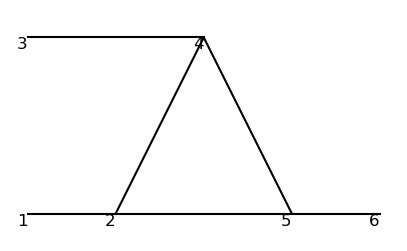
\includegraphics[width=0.7\textwidth]{plots/order3/order3_1to2/1.png}
        \caption{Diagram with a three-gluon loop.}
    \end{subfigure}%
    \begin{subfigure}[t]{0.5\textwidth}
        \centering
        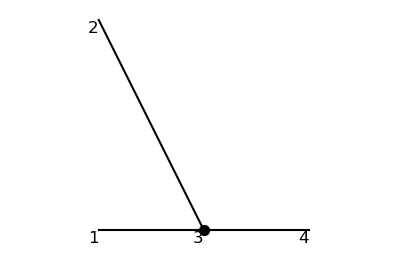
\includegraphics[width=0.7\textwidth]{plots/order3/order3_1to2/counterterms/1.png}
        \caption{Counterterm of the diagram}
    \end{subfigure}
    \caption{A example of a possible diagram, a third order contribution to the 
    process of three-gluon vertex, 1 gluon incoming and 2 gluons outgoing. (Outputs of 
    the programs.)}
    \label{fig:example_diagram}
\end{figure*}

Following the previous definitions, the diagram represent a process where a gluon
interacts in a third order process, forming a three-gluon loop, and 2 gluons are 
produced in the final state. Due to the presence of a loop, the diagram is
divergent, and a counterterm diagram is needed to deal with the divergence. This 
diagram is represented with a dot at the position of the loop, with the same 
external legs as the original diagram. 

\subsection{Order by order solutions.} \label{sec:orderbyorder_solutions}

The solution of the differential equations \eqref{eq:diff_order1} to \eqref{eq:diff_order3} 
and so on, without considering the multiplicative factors, and relative phases between
the terms, can be expressed as,

\begin{align}
    \mathcal{H}_{t1} & = \mathcal{H}_{01} \\
    \mathcal{H}_{t2} & = \mathcal{G}_{02} + \mathcal{H}_{01} 
    \mathcal{H}_{01}\\
    \mathcal{H}_{t3} & = \mathcal{G}_{03} + \mathcal{H}_{01} \mathcal{H}_{01}
    \mathcal{H}_{01} + \parenthesis{\mathcal{G}_{02} \mathcal{H}_{01} + 
    \mathcal{H}_{01} \mathcal{G}_{02}}\\
    \mathcal{H}_{t4} & = \mathcal{G}_{04} + \mathcal{H}_{01} \mathcal{H}_{01}
    \mathcal{H}_{01} \mathcal{H}_{01} + \parenthesis{\mathcal{G}_{02} 
    \mathcal{H}_{01} \mathcal{H}_{01} +  \mathcal{H}_{01} \mathcal{G}_{02}
    \mathcal{H}_{01} + \mathcal{H}_{01} \mathcal{H}_{01} \mathcal{G}_{02}} \nonumber\\
    & + \parenthesis{\mathcal{G}_{03} \mathcal{H}_{01} + \mathcal{H}_{01} 
    \mathcal{G}_{03} + \mathcal{G}_{02}\mathcal{G}_{02}}. \\
    &\vdots  \nonumber
\end{align}

This is an oversimplification of the solution, but it gives an idea of how the 
different solutions for each order are obtained. 

For instance, the diagrams for the first order is simply the canonical diagrams from
$\mathcal{H}_{01}$. As for the second order, it contains the canonical diagrams from 
the second order $\mathcal{G}_{02}$, and the product of the first order diagrams. The 
third order contains the canonical diagrams from the third order $\mathcal{G}_{03}$,
and the product of the first order, and second order canonical diagrams, as well as the 
product of exclusive first order diagrams. This way, we could rewrite the solution for 
each order in terms of the solution to the previous order,

\begin{align}
    \mathcal{H}_{t1} & = \mathcal{H}_{01} = \mathcal{G}_{01}, \\
    \mathcal{H}_{t2} & = \mathcal{G}_{02} + \mathcal{H}_{t1} \mathcal{G}_{01}, \\
    \mathcal{H}_{t3} & = \mathcal{G}_{03} + \mathcal{H}_{t1} \mathcal{G}_{02} + 
    \mathcal{H}_{t2} \mathcal{G}_{01}, \\
    \mathcal{H}_{t4} & = \mathcal{G}_{04} + \mathcal{H}_{t2} \mathcal{G}_{02} + 
    \mathcal{H}_{t1} \mathcal{G}_{03} + \mathcal{H}_{t3} \mathcal{G}_{01} \label{eq:sol_order4}\\
    \vdots & \nonumber
\end{align}

This way of writing the solution is useful to understand how the different
orders are related to each other, and how an iterative process can be used to
obtain the solution for each order.

\section{Case study: Gluons self-interactions} \label{sec:cases}

\subsection{Canonical Hamiltonian}

The Lagrangian density for the gluon fields is given by,
\begin{equation}
    \mathcal{L} = -\frac{1}{2}\text{tr}F^{\mu\nu}F_{\mu\nu},
\end{equation}
where $F^{\mu\nu}$ is the field strength tensor, defined as,
\begin{equation}
    F^{\mu\nu} = \partial^\mu A^\nu - \partial^\nu A^\mu + ig [A^\mu, A^\nu],
\end{equation}
and $A^\mu = A^{a\mu}t^a$, $t^a$ are the generators of the gauge group, and $g$ is the
coupling constant. Verifying the following relations,

\begin{equation}
    [t^a, t^b] = i f^{abc} t^c, \quad \text{tr}(t^a t^b) = \frac{1}{2} \delta^{ab}.
\end{equation}

We will be working in the gauge $A^+=0$, where the Lagrange equations constrain
the component $A^-$ to become 

\begin{equation}
    A^- = \frac{1}{\partial^+}2 \partial^\perp A^\perp - \frac{2}{\partial^{+2}} ig 
    \sbrackets{\partial^+ A^\perp, A^\perp}.
\end{equation}

In this way, the only degree of freedom left is the transverse component $A^\perp$.

As for the associated energy-momentum tensor,

\begin{equation}
    \mathcal{T}^{\mu\nu} = -F^{a\mu\alpha}\partial^\nu A^a_\alpha + 
    \frac{1}{4}g^{\mu\nu}F^{\alpha\beta} F_{\alpha\beta}.
\end{equation}

The Hamiltonian in FF quantization is obtained from integrating the component
$\mathcal{T}^{+-}$ of the energy-momentum tensor, over the hyperplane $x^+=0$. 

By working in the gauge $A^+=0$, the Hamiltonian density can be expressed as the sum of 
4 terms, as denoted in \cite{glazek_dynamics_2001}

\begin{equation}
    \mathcal{T}^{+-} = \mathcal{H}_{A^2} + \mathcal{H}_{A^3} +
    \mathcal{H}_{A^4} + \mathcal{H}_{[\partial AA]^2},
\end{equation}
with each of the terms, 

\begin{align}
    \mathcal{H}_{A^2} &= -\frac{1}{2} A^{\perp a} (\partial^\perp)^2 A^{\perp a}, \\
    \mathcal{H}_{A^3} &= g i \partial_\alpha A^a_\beta \sbrackets{A^\alpha, A^\beta}^a, \\
    \mathcal{H}_{A^4} &= -\frac{1}{4} g^2 \sbrackets{A_\alpha, A_\beta}^a
    \sbrackets{A^\alpha, A^\beta}^a, \\
    \mathcal{H}_{[\partial AA]^2} &= -\frac{1}{2} g^2 \sbrackets{i \partial^+ A^\perp,
    A^\perp}^a  \frac{1}{(i\partial^+)^2} \sbrackets{i\partial^+ A^\perp, A^\perp}^a.
\end{align}

Replacing $A^\mu$ with the operator $\hat{A}^\mu(x)$, defined by its Fourier composition
on the plane $x^+=0$,
\begin{equation}
    \hat{A}^\mu(x) = \sum _{\sigma c} \int [k] \sbrackets{t^c \epsilon^\mu_{k \sigma} 
    a_{k\sigma c}  e^{-ikx} + t^c \epsilon^{\mu*}_{k \sigma} 
    a^\dagger_{k\sigma c}  e^{ikx}}_{x^+=0},
\end{equation}
where $[k] = \theta(k^+) dk^+ d^2k^\perp / (16\pi^3k^+)$, $\epsilon^\mu_{k \sigma}$ 
are the polarization vectors, $t^c$ are the generators of the gauge group, and $a^\dagger_{k\sigma c}$, $a_{k\sigma c}$ are the 
creation and annihilation operators (particle operators), respectively. 


Substituting this expression into each term of the Hamiltonian densities, integrating
over space coordinates and taking into account the completeness and orthonormality 
of the polarization vectors, we obtain the following expression for the different
terms of the Hamiltonian \cite{QCDG}, 

\begin{align}
    H_{A^2} &= \sum_{\sigma c} \int [k] \frac{k^{\perp 2}}{k^+}a^\dagger_{k\sigma c}
    a_{k\sigma c}, \label{eq:H_A^2}\\
    H_{A^3} &= \sum_{123} \int [123] \slashed{\delta}(p^\dagger - p) \tilde{r}_{\Delta \delta}
    (3, 1) \sbrackets{gY_{123}a_1^\dagger a_2^\dagger a_3 + gY_{123}^*a_3^\dagger a_2 a_1},
    \label{eq:H_A^3}\\
    H_{A^4} &= \sum_{1234} \int [1234] \slashed{\delta}(p^\dagger - p) \frac{g^2}{4}
    \sbrackets{\parenthesis{\Xi_{A^4 1234} a_1^\dagger a_2^\dagger a_3^\dagger a_4 + h.c.}+ X_{A^4 1234} 
    a_1^\dagger a_2^\dagger a_3 a_4 }, \label{eq:H_A^4}\\
    H_{\sbrackets{\partial A A}^2} &= \sum_{1234} \int [1234] \slashed{\delta}
    (p^\dagger - p) g^2 \sbrackets{\parenthesis{\Xi_{\sbrackets{\partial A A}^2 1234}
    a_1^\dagger a_2^\dagger a_3^\dagger a_4 + h.c.} + X_{\sbrackets{\partial A A}^2 
    1234} a_1^\dagger a_2^\dagger a_3 a_4 } \label{eq:H_partial}.
\end{align}

\subsection{Canonical diagrams}
The canonical diagrams are the diagrams that are obtained from the canonical
Hamiltonian, and are the starting point to obtain the diagrams of higher order.

Following the creation and annihilation operators in the different terms of the 
Hamiltonian, we can distinguish the different types of process that are being
considered. 

Starting from the term $H_{A^2}$ in equation \eqref{eq:H_A^2}, we can see that this 
a particle of certain momentum $k$ is annihilated and created, producing the same
particle. This corresponds to the kinetic term of the Hamiltonian, and the diagram 
will be a line with the same color/type of particle in both ends. Since it is an 
order 0 term, it will not contribute to the perturbative expansion.

Figure \ref{fig:cannonical1} shows the two types of first-order diagrams 
(one gluon splitting into two, and its inverse process of two gluons merging into one),
corresponding to the term $H_{A^3}$ in equation \eqref{eq:H_A^3}.
This process is represented by a diagram with 3 external legs, and 1 vertex, thus a 
first order term.

\begin{figure*}[h!]
    \centering
    \begin{subfigure}[t]{0.33\textwidth}
        \centering
        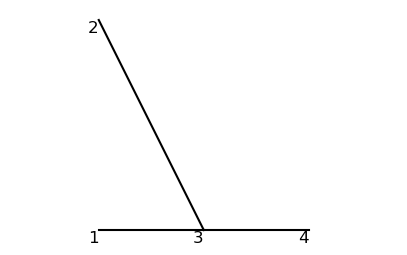
\includegraphics[width=\textwidth]{plots/canonical/order1/1.png}
        \caption{ }
    \end{subfigure}%
    \begin{subfigure}[t]{0.33\textwidth}
        \centering
        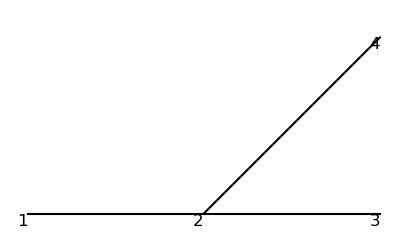
\includegraphics[width=\textwidth]{plots/canonical/order1/2.png}
        \caption{ }
    \end{subfigure}
    \caption{Canonical diagrams of order 1}
    \label{fig:cannonical1}
\end{figure*}

\newpage

The term $H_{A^4}$ in equation \eqref{eq:H_A^4} is a four-gluon vertex, where either
1 gluon is annihilated, and 3 gluons are created, 3 gluons are annihilated, and
1 gluon is created, or 2 gluons are annihilated, and 2 gluons are created. However, 
since we are building higher-order diagrams from lower-order ones, it’s convenient 
to treat the four-gluon vertex as a combination of two three-gluon vertices. Meaning that 
for the process where one gluon goes to 3 gluons, we consider the process as, 
one gluon being annihilated, and 2 gluons are created, then one of the
created gluons is annihilated, and 2 gluons are created, producing a total of 3 gluons
in the final state. The same applies for the process where 3 gluons are annihilated.
This way, these diagrams have 2 vertices, and thus a second order term, that 
can be obtained from the product of the canonical first order diagrams, so we 
will not consider them as a new canonical diagrams, but rather as a result that will
be obtained during the perturbative expansion.

The $H_{\sbrackets{\partial A A}^2}$ term represents an instantaneous gluon exchange 
(often drawn as a vertical line in light-front diagrams). This allows to consider processes where a gluon is annihilated, and 3 gluons are created, to a 
pair of three-gluon vertices, similar to $H_{A^4}$. The main difference is that
the interaction is instantaneous, meaning that the gluon is annihilated, and the
3 gluons are created at the same time, without any time delay between them.

In our program, we treat this as a special kind of ‘virtual particle’ (drawn with 
a dotted line) to include it in the same diagram framework. Similar to the 
term $H_{A^4}$, this term is a four-gluon vertex, except for the instantaneous 
interaction. 

The different sum terms in the equation \eqref{eq:H_partial} indicate the different 
processes that can be considered, the first term $\Xi_{\sbrackets{\partial A A}^2 1234}$
indicate the process where 1 gluon is annihilated, and 3 gluons are created, as shown in
figure \ref{fig:cannonical2_1to3}. The second term $\Xi_{\sbrackets{\partial A A}^2 1234}^*$
indicate the hermitian conjugate of the first term, where 3 gluons are annihilated, and
1 gluon is created, as shown in figure \ref{fig:cannonical2_3to1}. The third term
$X_{\sbrackets{\partial A A}^2 1234}$ indicate the process where 2 gluons are annihilated,
and 2 gluons are created, as shown in figure \ref{fig:cannonical2_2to2}.

\begin{figure*}[h!]
    \centering
    \begin{subfigure}[t]{0.33\textwidth}
        \centering
        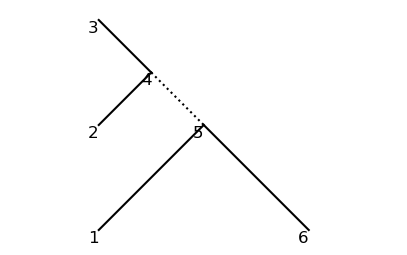
\includegraphics[width=\textwidth]{plots/canonical/order2/1.png}
        \caption{ }
    \end{subfigure}%
    \begin{subfigure}[t]{0.33\textwidth}
        \centering
        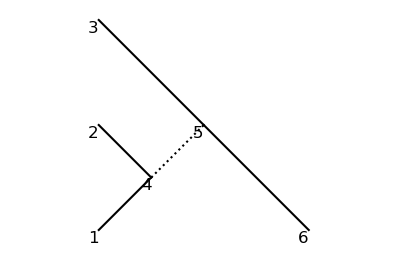
\includegraphics[width=\textwidth]{plots/canonical/order2/2.png}
        \caption{ }
    \end{subfigure}
    \begin{subfigure}[t]{0.33\textwidth}
        \centering
        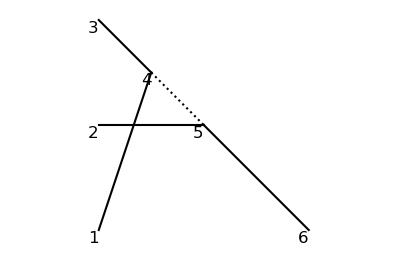
\includegraphics[width=\textwidth]{plots/canonical/order2/3.png}
        \caption{ }
    \end{subfigure}
    \caption{Canonical diagrams of order 2, for the term $\Xi_{\sbrackets{\partial AA}^2}$, 
    where one gluon is annihilated, and 3 gluons are created.}
    \label{fig:cannonical2_1to3}
\end{figure*}

\begin{figure*}[h!]
    \centering
    \begin{subfigure}[t]{0.33\textwidth}
        \centering
        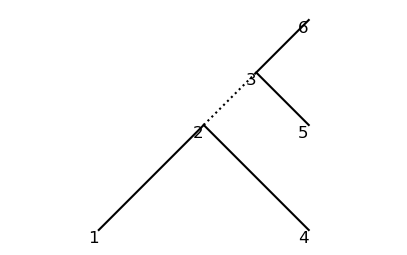
\includegraphics[width=\textwidth]{plots/canonical/order2/9.png}
        \caption{ }
    \end{subfigure}%
    \begin{subfigure}[t]{0.33\textwidth}
        \centering
        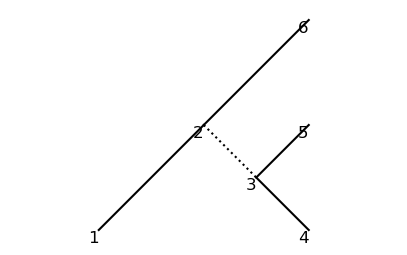
\includegraphics[width=\textwidth]{plots/canonical/order2/10.png}
        \caption{ }
    \end{subfigure}
    \begin{subfigure}[t]{0.33\textwidth}
        \centering
        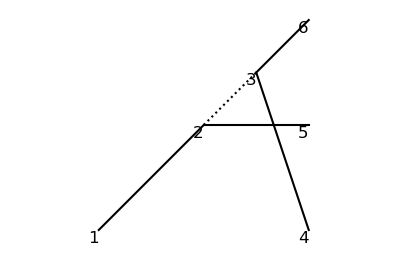
\includegraphics[width=\textwidth]{plots/canonical/order2/11.png}
        \caption{ }
    \end{subfigure}
    \caption{Canonical diagrams of order 2, for the term hermitian conjugate of 
    $\Xi_{\sbrackets{\partial AA}^2}$, where 3 gluons are annihilated, and
    1 gluon is created.}
    \label{fig:cannonical2_3to1}
\end{figure*}

\begin{figure*}[h!]
    \centering
    \begin{subfigure}[t]{0.24\textwidth}
        \centering
        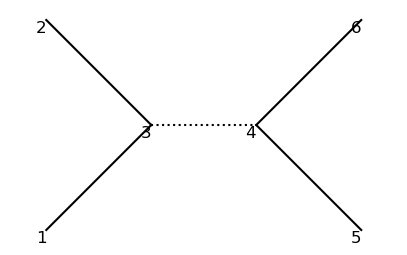
\includegraphics[width=\textwidth]{plots/canonical/order2/4.png}
        \caption{ }
    \end{subfigure}%
    \begin{subfigure}[t]{0.24\textwidth}
        \centering
        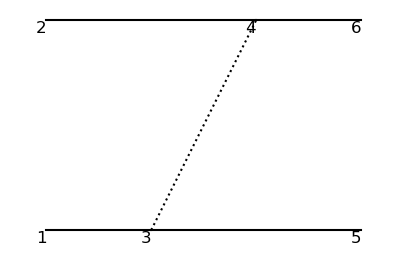
\includegraphics[width=\textwidth]{plots/canonical/order2/5.png}
        \caption{ }
    \end{subfigure}
    \begin{subfigure}[t]{0.24\textwidth}
        \centering
        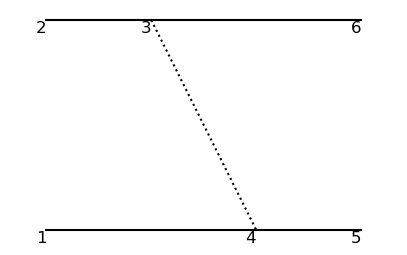
\includegraphics[width=\textwidth]{plots/canonical/order2/6.png}
        \caption{ }
    \end{subfigure}
    \begin{subfigure}[t]{0.24\textwidth}
        \centering
        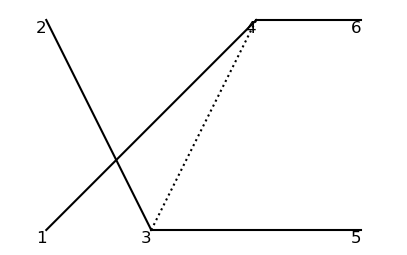
\includegraphics[width=\textwidth]{plots/canonical/order2/7.png}
        \caption{ }
    \end{subfigure}
    \begin{subfigure}[t]{0.24\textwidth}
        \centering
        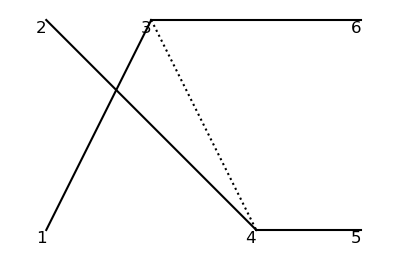
\includegraphics[width=\textwidth]{plots/canonical/order2/8.png}
        \caption{ }
    \end{subfigure}
    \caption{Canonical diagrams of order 2, for the term $X_{\sbrackets{\partial AA}^2}$, 
    where 2 gluons are annihilated, and 2 gluons are created.}
    \label{fig:cannonical2_2to2}
\end{figure*}

\newpage

The combination of all these diagrams, are the canonical diagrams of order 2.
Together with the diagrams of order 1, figure \ref{fig:cannonical1},
they form the basis of the perturbative expansion of the Hamiltonian, and the
starting point to obtain the diagrams of higher order.

As we can see, in the case of QCD, there are only canonical diagrams of order 1 and 2, 
then referring to the framework laid out in section \ref{sec:orderbyorder_solutions}, 
from order 3  and onwards, the diagrams only depend explicitly on the diagrams of 
previous order, as well as the order 1, and the order 2 canonical diagrams.

For example, in Eq. \eqref{eq:sol_order4}, the solution at order $4$, $\mathcal{H}_{t4}$ consists of 
$\mathcal{H}_{t 3}$ and the canonical diagrams, thus eliminating the term with $\mathcal{G}_{04}$ and
$\mathcal{H}_{t1}\mathcal{G}_{03}$, since they are not present in the QCD theory.
This simplifies the number of diagrams that can be obtained at higher orders,
and making the diagrams have the form,

\begin{align}
    \mathcal{H}_{t1} & = \mathcal{H}_{01} = \mathcal{G}_{01}, \\
    \mathcal{H}_{t2} & = \mathcal{G}_{02} + \mathcal{H}_{t1} \mathcal{G}_{01}, \\
    \mathcal{H}_{t3} & =  \mathcal{H}_{t1} \mathcal{G}_{02} + 
    \mathcal{H}_{t2} \mathcal{G}_{01}, \\
    \mathcal{H}_{t4} & =  \mathcal{H}_{t2} \mathcal{G}_{02} + \mathcal{H}_{t3} \mathcal{G}_{01}\\
    \mathcal{H}_{t5} & =  \mathcal{H}_{t3} \mathcal{G}_{02} + \mathcal{H}_{t4} \mathcal{G}_{01} \\
    \vdots & \nonumber\\
    \mathcal{H}_{tn} &=  \mathcal{H}_{t(n-1)} \mathcal{G}_{02} +
    \mathcal{H}_{t(n-2)} \mathcal{G}_{01} \quad \text{for } n \geq 3.
\end{align}

Obtaining a simpler recursive relation to obtain the diagrams of higher order,
that can be implemented in a program to obtain the diagrams of higher order.

\newpage

\section{Code implementation} \label{sec:code}

The code is implemented in Python, but the general method can be applied to any 
programming language. The program is designed to be modular, and applicable to
other theories, by considering some minor modifications and changing the canonical
diagrams. These modifications are not implemented yet, and remain to be tested.

\subsection{Diagrams definition}

The diagrams are defined by 2 arrays, 
\begin{itemize}
    \item Points: arrays of dimension $N \times 2$, where $N$ is the number of 
    points in the diagram, each point is defined by its coordinates $(x,y)$.
    \item Paths: arrays of dimension $M \times N^\prime \times 2$, where $M$ is the
    number of different types of particles to consider in the theory, $N^\prime$ 
    is the number of paths for each types of particle in the diagram, and $2$ indicate
    the points to connect.
\end{itemize}

This way of defining the diagrams is analogous to the way of defining the undirected 
graphs in the graph theory, where the points are the vertices and the paths are the 
edges. 

In the case of gluon interactions, although only 1 type of particle is present, the
instantaneous interactions have to be considered. This is done by defining this 
interaction as a new type of virtual particle in the program.


\subsection{Order by order procedure}

To calculate the diagrams of higher order, the code follows the order by order 
procedure described in Section \ref{sec:theoretical_background}. Having only the
canonical diagrams, the program aims to obtain all the possible diagrams of an order
that contribute to a certain process, discarding the other diagrams.

The program would follow a recursive procedure, where the diagrams of order $n$ are
obtained from the diagrams of order $n-1$ and $n-2$, in a procedure that can be outlines
as follows,

\begin{enumerate}
    \item Start with the canonical diagrams of order 1 and 2.
    \item For each order $n$, starting from 3, do the following,
    \begin{enumerate}
        \item Generate all possible combinations of diagrams of order $n-1$ with
        order 1, and $n-2$ with order 2.
        \item For each combination, check if it is a valid diagram for the process
        being considered.
        \item If it is a valid diagram, add it to the list of diagrams for order $n$.
    \end{enumerate}
    \item After generating all the diagrams of order $n$, check for equivalent diagrams,
    and add their contributions to the list of diagrams.
    \item If the order is greater than 2, check for loops, and add the counterterms 
    to the list of diagrams.
    \item Repeat the process for the next order, until the desired order is reached.
\end{enumerate}

The step 3 is fundamental in order to reduce the number of diagrams that needs to 
be used to calculate the next order. This procedure is the most time-consuming process 
of the program, needing a search algorithm to find the equivalent diagrams, meaning 
that as the order increases, the number of diagrams increases exponentially, and the 
time to find the equivalent diagrams increases exponentially too. 

Although the process of finding the equivalent diagrams is time-consuming, it is
fundamental to reduce the global computational time. Since the number of diagrams 
tend to decrease by 1 to 2 orders of magnitude, depending on the order and the number of
particles in the process. This way reduces the time needed to calculate the
diagrams of the next order, so at the grand scale, the time needed to calculate
the diagrams of till a certain order is reduced by performing the search algorithm in
between the orders.


\subsection{Applied to gluons self-interactions} \label{sec:applied_gluons}
Although in this thesis the focus is on the gluons and its self-interactions, 
and considering only one type of particle, there are tests that can be done to 
check the validity of the program for multiple types of particles. Thanks to
the instantaneous interactions, the program can be adapted to consider this 
type of interactions as a new type of particles, and thus check for bugs or other 
issues that may arise when considering multiple types of particles.

This approach comes with its own problems. By considering an instantaneous 
process as a new type of particles, this process need to respect the time 
evolution of the system, meaning that in the eyes of the program, the 
instantaneous interaction is no longer instantaneous, but rather a process that
happens in a certain time interval. 

Nonetheless, this is a valid approach to consider the instantaneous interactions, 
since no possible diagrams will be lost, rather equivalent diagrams will be 
obtained, without the program being aware of it, and it rests on the user to
identify these equivalences. 

For lower orders, this approach works well, since the number of diagrams is
manageable, but at higher orders, this is a problem that needs to be addressed in 
the future, and a general fix to the problem will be implemented in the program.

\newpage

\section{Diagrams obtained} \label{sec:diagrams}

In this section, we will present the diagrams obtained from the program. At 
each order, we will consider the types of processes that is the most relevant.


\subsection{Order 3}

Considering the three-gluon vertex, the process of 1 gluon going to 2 gluons, up till 
order 3, the diagrams obtained from the program are shown in the figures 
\ref{fig:order3_1to2} and \ref{fig:order3_1to2/counterterms}.

\begin{figure*}[h!]
    \centering
    \begin{subfigure}[t]{0.24\textwidth}
        \centering
        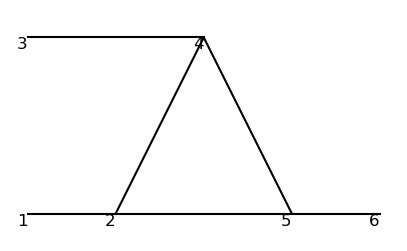
\includegraphics[width=\textwidth]{plots/order3/order3_1to2/1.png}
        \caption{ }
    \end{subfigure}%
    \hfill
    \begin{subfigure}[t]{0.24\textwidth}
        \centering
        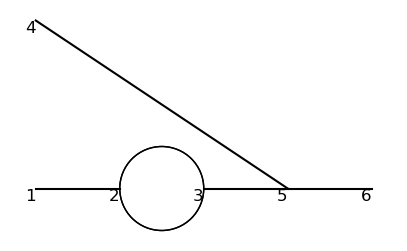
\includegraphics[width=\textwidth]{plots/order3/order3_1to2/2.png}
        \caption{ }
    \end{subfigure}
    \hfill
    \begin{subfigure}[t]{0.24\textwidth}
        \centering
        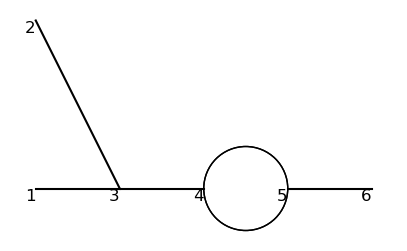
\includegraphics[width=\textwidth]{plots/order3/order3_1to2/3.png}
        \caption{ }
    \end{subfigure}
    \hfill
    \begin{subfigure}[t]{0.24\textwidth}
        \centering
        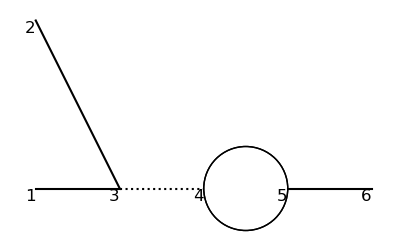
\includegraphics[width=\textwidth]{plots/order3/order3_1to2/4.png}
        \caption{ }
    \end{subfigure}
    \hfill
    \begin{subfigure}[t]{0.24\textwidth}
        \centering
        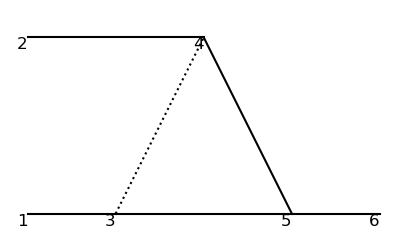
\includegraphics[width=\textwidth]{plots/order3/order3_1to2/5.png}
        \caption{ }
        \label{fig:order3_1to2/5}
    \end{subfigure}
    \hfill  
    \begin{subfigure}[t]{0.24\textwidth}
        \centering
        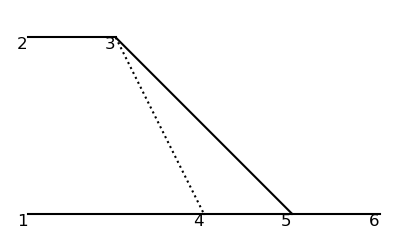
\includegraphics[width=\textwidth]{plots/order3/order3_1to2/6.png}
        \caption{ }
        \label{fig:order3_1to2/6}
    \end{subfigure}
    \hfill
    \begin{subfigure}[t]{0.24\textwidth}
        \centering
        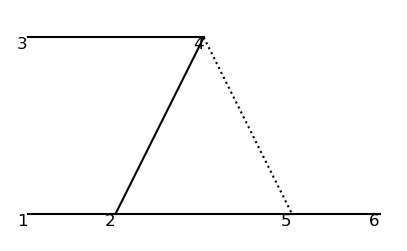
\includegraphics[width=\textwidth]{plots/order3/order3_1to2/7.png}
        \caption{ }
    \end{subfigure}
    \hfill 
    \begin{subfigure}[t]{0.24\textwidth}
        \centering
        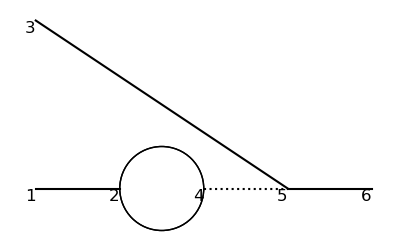
\includegraphics[width=\textwidth]{plots/order3/order3_1to2/8.png}
        \caption{ }
    \end{subfigure}
    \caption{Diagrams of third order, contributing to the three-gluon vertex.}
    \label{fig:order3_1to2}
\end{figure*}

\begin{figure*}[h!]
    \centering
    \begin{subfigure}[t]{0.24\textwidth}
        \centering
        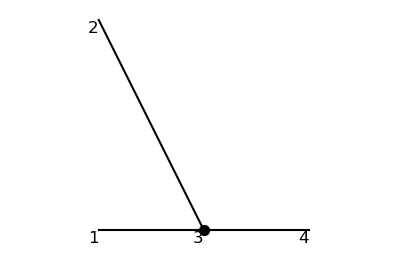
\includegraphics[width=\textwidth]{plots/order3/order3_1to2/counterterms/1.png}
        \caption{ }
    \end{subfigure}%
    \hfill
    \begin{subfigure}[t]{0.24\textwidth}
        \centering
        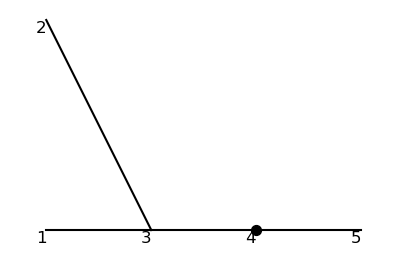
\includegraphics[width=\textwidth]{plots/order3/order3_1to2/counterterms/2.png}
        \caption{ }
    \end{subfigure}
    \hfill
    \begin{subfigure}[t]{0.24\textwidth}
        \centering
        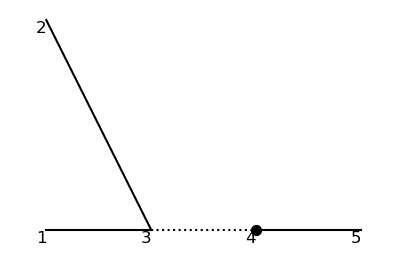
\includegraphics[width=\textwidth]{plots/order3/order3_1to2/counterterms/3.png}
        \caption{ }
    \end{subfigure}
    \hfill
    \begin{subfigure}[t]{0.24\textwidth}
        \centering
        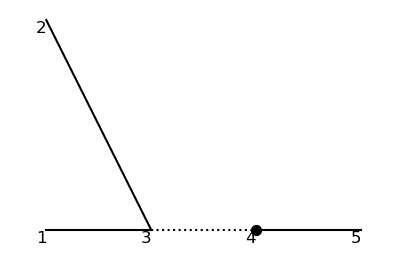
\includegraphics[width=\textwidth]{plots/order3/order3_1to2/counterterms/4.png}
        \caption{ }
        \label{fig:order3_1to2/counterterms/4}
    \end{subfigure}
    \hfill
    \begin{subfigure}[t]{0.24\textwidth}
        \centering
        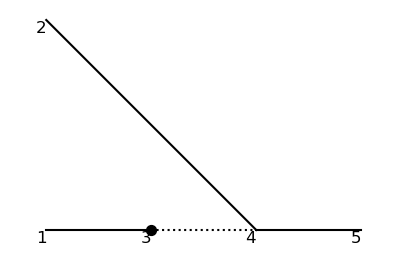
\includegraphics[width=\textwidth]{plots/order3/order3_1to2/counterterms/5.png}
        \caption{ }
        \label{fig:order3_1to2/counterterms/5}
    \end{subfigure}
    \caption{Counterterms to the diagrams of third order in figure \ref{fig:order3_1to2}}
    \label{fig:order3_1to2/counterterms}
\end{figure*}


In the figure \ref{fig:order3_1to2} we can see the diagrams obtained for the process
of 1 gluon going to 2 gluons, with the corresponding counterterms in figure
\ref{fig:order3_1to2/counterterms}. 

Depending on the types of particles in the process, we can deduce the origin of the 
different diagrams. With the once having dotted lines, and thus coming from the second
order term canonical diagrams $H_{\sbrackets{\partial A A}^2}$, combined with a first 
order term canonical diagram $H_{A^3}$. While the diagrams without dotted lines
come solely from the first order term canonical diagrams $H_{A^3}$

Referring to the problems mentioned in Section \ref{sec:applied_gluons}, the diagrams 
with dotted lines are instantaneous interactions, but the program considers them
as a new type of particle, there are some artifacts that arise from this
approach. For instance, the diagrams \ref{fig:order3_1to2/5} and \ref{fig:order3_1to2/6} are really the same 
diagram, due to instant process being instantaneous. For any other particle, these 
2 diagrams would be different, due to the importance of the order in the interactions,
so the program is kept to consider them as different, to not lose generality.

Other artifact of the program occur for the diagrams \ref{fig:order3_1to2/counterterms/4} and
\ref{fig:order3_1to2/counterterms/5}, which are counterterms added to cancel the divergences
in the canonical diagrams. These counterterms are already considered in the canonical diagrams, 
and thus not needed to be added again. But due to the way the program is implemented,
it adds counterterms to all loop divergences in the diagrams.

Comparing with the 3rd order contribution diagrams in \cite{QCDG}, the same diagrams
for the three-gluon vertex are obtained, proving the validity of the program to reproduce the same results.



\subsection{Order 4}

In a non abelian theory such as QCD, the gluons interact with themselves, thus making 
bound states formed by exclusively gluons, glueballs, possible. 

Considering one of such glueball states, the process of 2 gluons going to 2 gluons, the program
produces about 100 diagrams, with the corresponding counterterms. All the diagrams are
not shown here, since they are too many to be included in this document. But let's 
discuss some of the most interesting diagrams.

\begin{figure*}[h!]
    \centering
    \begin{subfigure}[t]{0.33\textwidth}
        \centering
        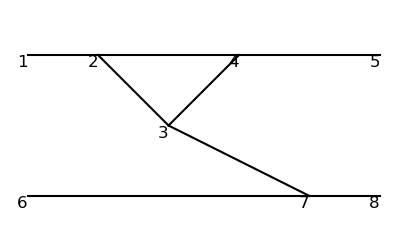
\includegraphics[width=\textwidth]{plots/order4/1.png}
        \caption{ }
    \end{subfigure}%
    \begin{subfigure}[t]{0.33\textwidth}
        \centering
        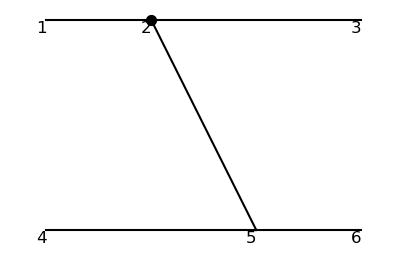
\includegraphics[width=\textwidth]{plots/order4/counterterms/1.png}
        \caption{ }
    \end{subfigure}
    \caption{Diagrams of fourth order,}
    \label{fig:order4/1}
\end{figure*}

Starting at order 4, the distinct non-abelian nature of the QCD is present, since 
the gluons interact with themselves, creating diagrams not possible in abelian theories, 
such as QED. One of such processes is shown in the figure \ref{fig:order4/1}, where 2 gluons
interact with each other.

\newpage


\subsection{Higher orders}

At higher orders, the diagrams become more complex, and the number of diagrams scale 
exponentially. Is here where the power of the program is shown. 

\begin{table} [h!]
    \centering
    \begin{tabular}{|c|c|c|}
        \hline
        Order & Unique diagrams & Computational time (s)\\
        \hline
        2  & 16 & 0.150\\
        3  & 76 & 0.198\\
        4  & 612 & 1.166\\
        5  & 5871  & 10.935\\
        6  & 65000  & 157.121\\
        \hline
    \end{tabular}
    \caption{Number of diagrams obtained by the program at each order, and the Computational
    time taken to calculate the diagrams.}
    \label{tab:diagrams}
\end{table}

\newpage

\section{Conclusions and future work} \label{sec:conclusions}


In this thesis, we have presented a program that implements the RGPEP to obtain the
diagrams of the gluons self-interactions, and the perturbative expansion of the
Hamiltonian. The program is able to obtain the diagrams of higher order, starting
from the canonical diagrams, and using the order by order procedure.
The program is modular, and can be adapted to other theories, by changing the
canonical diagrams and the types of particles considered.
The program has been tested with the gluons self-interactions, and has been able to
obtain the diagrams of higher order, with the corresponding counterterms to cancel
the divergences produced in the process. The program has been able to reproduce the
diagrams obtained in the literature, proving its validity to obtain the diagrams of
higher order in the perturbative expansion of the Hamiltonian.

The program is able to obtain the diagrams of higher order, but there are still
some issues that need to be addressed, such as the artifacts produced by the
instantaneous interactions, and the time taken to calculate the diagrams at higher
orders. 

The program is still in development, and there are many improvements that can
be made to optimize the process of obtaining the diagrams. Other main issue to 
address is the counting of the diagrams, as the program is able to obtain the diagrams, 
but it does not output the symmetry factor correctly, due to the problems with the factors 
associated to the canonical diagrams, and the counterterms, as well as the method
used to find the diagrams that prioritize ensuring that no diagrams are lost, rather than
ensuring that the symmetry factor is correct.

As future work, we plan to fix the issues mentioned above, and to implement and 
test the program with other theories, and more types of particles, particularly
considering the quarks and antiquarks, in the general case of QCD. 

\section{Acknowledgements}

% Referencias %%%%%%%%%%%%%%%%%%%%%%%%%%%%%%%%%%%%%%%%%%%%%%%%%%%%%%%%%%%%%%%%%
\newpage

\bibliography{references} % Entries are in the references.bib file

\end{document}

